\documentclass[11pt]{article}

% ---------- Packages ----------
\usepackage[a4paper,margin=1in]{geometry}
\usepackage{lmodern}
\usepackage{graphicx}
\usepackage{float}
\usepackage{microtype}
\usepackage{amsmath,amssymb}
\usepackage{placeins}
\usepackage{booktabs}
\usepackage{fontawesome5}
\usepackage{hyperref}
\usepackage{caption}
\usepackage{subcaption}
\usepackage[superscript]{cite}
\usepackage{array}
\usepackage{enumitem}
\usepackage{setspace}
\usepackage{tabularx}   
\onehalfspacing

% TikZ for the pipeline figure
\usepackage{tikz}
\usetikzlibrary{arrows.meta,positioning}

\setcounter{tocdepth}{2}

% ---------- Metadata ----------
\hypersetup{
    pdftitle={GraFT: Alignment-Free Detection of Horizontal Gene Transfer Candidates via Protein Similarity Graphs and Anomaly Scoring},
    pdfauthor={Roee Tekoah, Noam Korkos},
    pdfsubject={Horizontal Gene Transfer detection using graph-based analysis},
    pdfkeywords={GraFT, HGT, Horizontal Gene Transfer, k-mer, graph analysis, anomaly scoring}
}

\title{\textbf{\LARGE GraFT: Alignment-Free Detection of HGT Candidates}\\[6pt]
{\large via Protein Similarity Graphs and Anomaly Scoring}}
\author{}
\date{}

\begin{document}
\maketitle
\vspace{-52pt}

\begin{center}
\renewcommand{\arraystretch}{1.15}
\setlength{\tabcolsep}{10pt}

\begin{tabular}{c@{\hspace{2.8cm}}c}
{\normalsize\textbf{Roee Tekoah}} &
{\normalsize\textbf{Noam Korkos}} \\[2pt]
\footnotesize\texttt{roee.tekoah@mail.huji.ac.il} &
\footnotesize\texttt{noam.korkos@mail.huji.ac.il}
\end{tabular}

\vspace{16pt}

{\small\itshape
The Rachel and Selim Benin School of Computer Science and Engineering\\
The Hebrew University of Jerusalem
}\\[8pt]
\faGithub\ \href{https://github.com/roeetekoah/GraFT/}{\texttt{Code, Docs \& Online Supplementary Material}}\\[10pt]
{\small February 2026}
\end{center}

\begin{abstract}
Horizontal gene transfer (HGT) is a major driver of microbial evolution, enabling rapid acquisition of adaptive functions such as antibiotic resistance and novel metabolic capabilities. Detecting HGT at scale remains challenging due to the computational cost and complexity of alignment and phylogeny-based methods. We present GraFT (Graph-based Finder of Transfers), a scalable, alignment-free pipeline for identifying HGT candidates in large protein collections using sparse protein similarity graphs and graph-based anomaly analysis. Proteins are compared via \textit{k}-mer overlap, normalized using robust statistics to account for species-specific background similarity, and embedded in a graph structure that enables detection of structurally anomalous cross-species similarity patterns. Applying GraFT to RefSeq bacterial proteins ($\approx$324,000 proteins across 50 species) reveals distinct connectivity regimes---including dense multi-taxa exchange modules, chained transfer-like structures, and localized high-confidence bridges---each corresponding to candidate HGT events with known biological significance. Our results demonstrate that graph-based structural context provides a powerful and interpretable signal for prioritizing HGT candidates suitable for downstream biological validation. We present the full formal scoring derivation alongside all hyperparameters, enabling complete reproducibility and transparent inspection of the ranking framework.
\end{abstract}

\setlength{\textfloatsep}{10pt}
\setlength{\floatsep}{8pt}
\setlength{\intextsep}{8pt}

\tableofcontents
\newpage

% =========================
% 1. Introduction
% =========================
\section{Introduction}

\subsection{Background}
\label{subsec:background}

Horizontal gene transfer (HGT) is a central driver of microbial evolution, enabling bacteria to share functional genes directly with other living organisms rather than relying solely on vertical inheritance\cite{KooninMakarova,Soucy2015}. This process allows genes to move between organisms regardless of phylogenetic distance, creating cases where a gene in one species is unexpectedly similar to a gene in a distantly related taxon. HGT underlies the rapid spread of antibiotic resistance across bacterial populations and the emergence of novel pathogens, making its detection a problem of significant biomedical importance\cite{Davies2000,Ochman2000,Frost2005}.

The main biological mechanisms by which HGT occurs are illustrated in Figure~\ref{fig:hgt-example}: conjugation (direct cell-to-cell transfer of plasmids), transformation (uptake of environmental DNA), and transduction (phage-mediated gene transfer). These pathways differ in their host-range specificity and the types of genes they typically move, but all can transfer functional genes---including antibiotic resistance determinants, toxins, surface modification enzymes, and novel metabolic enzymes---between phylogenetically distant bacteria.

\begin{figure}[H]
    \centering
    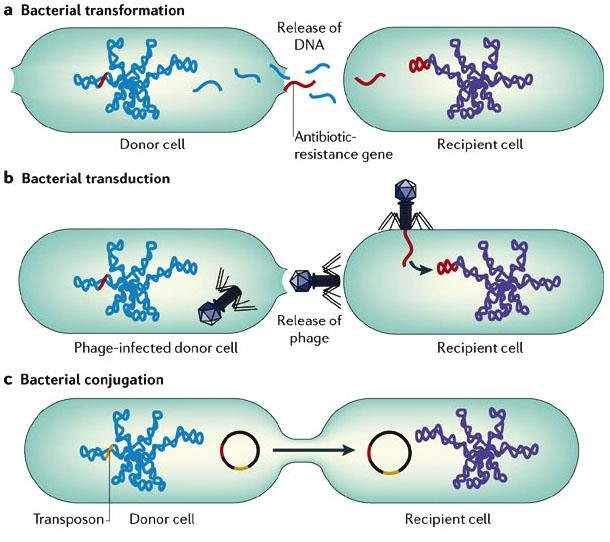
\includegraphics[width=0.55\textwidth]{figures/HGTExample.png}
    \caption{Biological mechanisms underlying horizontal gene transfer (HGT): conjugation, transformation, and transduction. From \href{https://www.researchgate.net/figure/Schematic-of-three-process-of-Horizontal-Gene-Transfer_fig2_277076640}{\textit{Nature Microbiology, \textcopyright{} 2006 Nature Publishing Group}}}
    \label{fig:hgt-example}
\end{figure}

However, high sequence similarity across distant taxa is not unique to HGT. Such patterns may also arise from strong functional conservation, heterogeneous evolutionary rates, gene loss in intermediate lineages, convergent evolution, or annotation and assembly artifacts\cite{Dilucca2018}. Distinguishing genuine transfer events from these confounders is a central challenge in the field.

Established approaches for detecting HGT rely on either phylogenetic incongruence---comparing gene trees to species trees---which is computationally intensive and sensitive to alignment quality and tree topology errors\cite{Ragan2001,Philippe2011,MishraLercher2025}---or on simpler heuristics such as nucleotide composition anomalies (GC content, codon usage) that can be noisy and miss recently transferred genes before amelioration has occurred. Large curated resources such as NCBI RefSeq motivate scalable screening methods that prioritize suspicious cross-species similarities for downstream validation\cite{OLeary2016}.

\subsection{Contributions}

We present GraFT, an alignment-free framework for large-scale HGT candidate discovery based on sparse protein similarity graphs. Our contributions are threefold. First, we introduce a \textbf{species-pair--aware normalization scheme} based on robust statistics (median and MAD) that calibrates cross-species similarity relative to heterogeneous background conservation levels, without requiring any explicit phylogenetic reconstruction. Second, we combine local anomaly evidence with graph-structural features in a \textbf{gated, component-aware ranking framework} that suppresses generic conserved proteins while prioritizing structurally informative candidates; we provide the full formal derivation of this scoring framework in Section~\ref{sec:scoring}. Third, we demonstrate that sparse similarity graphs reveal \textbf{distinct and interpretable connectivity regimes}---dense multi-taxa modules, chained topologies, and localized bridge structures---each consistent with different HGT-like transfer patterns, which we validate against the biological literature.

Unlike global-threshold similarity approaches, our framework explicitly calibrates similarity relative to species-pair baselines and integrates structural graph context into candidate ranking, enabling it to distinguish genuinely anomalous cross-species edges from those expected given the background divergence of each species pair.

% =========================
% 2. Data
% =========================
\section{Data}

\subsection{Data Source and Species Selection}

We constructed our dataset from the NCBI RefSeq protein database\cite{OLeary2016,RefSeqGenome}, focusing on a curated set of bacterial species. Assembly metadata were obtained from the RefSeq assembly summary and filtered to retain high-quality genomes at Complete Genome or Chromosome level, prioritizing reference and representative assemblies. Taxonomic lineage information was retrieved for each species from the NCBI Taxonomy database\cite{NCBITaxonomy}.

To control dataset size, we selected up to two assemblies per species using a deterministic ranking criterion. While this choice ensured manageable scale and consistent annotation quality, it introduced some redundancy due to near-identical assemblies for the same species; we discuss this limitation in Section~\ref{subsec:redundancy}.

\subsection{Protein Extraction and Preprocessing}

Protein FASTA files were downloaded from RefSeq and parsed into a unified table containing protein identifiers, species labels, and sequence lengths. Proteins shorter than 50 amino acids were excluded to reduce spurious similarity arising from short or low-complexity sequences. The final dataset contains approximately 324,000 proteins across 50 species spanning 19 taxonomic families. The selected 50 species provide a taxonomically diverse testbed while remaining computationally tractable; scaling to larger collections is enabled by the sparsity and modular design of GraFT.

% =========================
% 3. Method
% =========================
\section{Method}

An overview of the full pipeline is shown in Figure~\ref{fig:pipeline_overview}.

\begin{figure}[p]
\centering
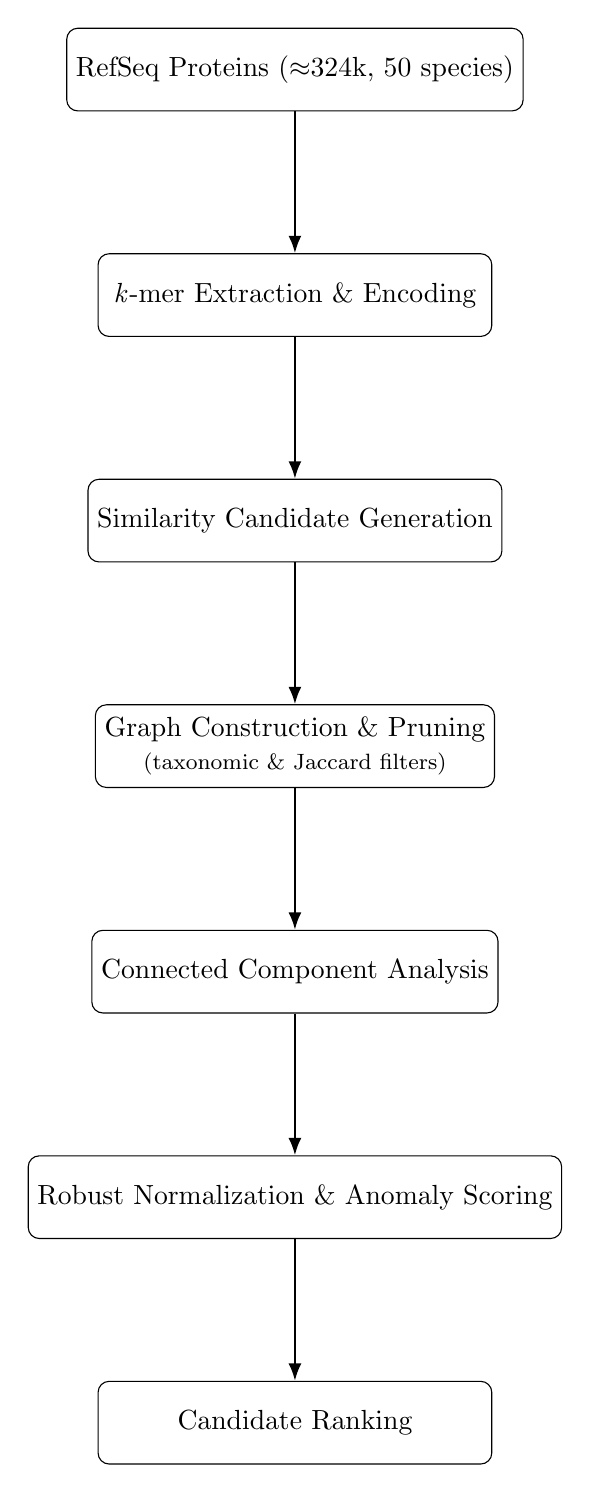
\begin{tikzpicture}[
    node distance=1.8cm,
    box/.style={draw, rectangle, rounded corners, align=center,
                minimum width=5.0cm, minimum height=1.05cm},
    arrow/.style={-{Latex[length=2.2mm]}, thick}
]
\node[box] (data)  {RefSeq Proteins ($\approx$324k, 50 species)};
\node[box, below=of data]  (kmers) {\textit{k}-mer Extraction \& Encoding};
\node[box, below=of kmers] (cand)  {Similarity Candidate Generation};
\node[box, below=of cand]  (prune) {Graph Construction \& Pruning\\{\footnotesize (taxonomic \& Jaccard filters)}};
\node[box, below=of prune] (comp)  {Connected Component Analysis};
\node[box, below=of comp]  (score) {Robust Normalization \& Anomaly Scoring};
\node[box, below=of score] (rank)  {Candidate Ranking};

\draw[arrow] (data)  -- (kmers);
\draw[arrow] (kmers) -- (cand);
\draw[arrow] (cand)  -- (prune);
\draw[arrow] (prune) -- (comp);
\draw[arrow] (comp)  -- (score);
\draw[arrow] (score) -- (rank);
\end{tikzpicture}
\caption{Overview of the GraFT HGT candidate detection pipeline. Protein sequences are represented using \textit{k}-mers to generate cross-species similarity candidates. A multi-step pruning procedure controls graph density by retaining high-confidence, taxonomically informative edges. Robust normalization and graph-based anomaly scoring are then applied across connected components to identify and rank candidate HGT-related proteins.}
\label{fig:pipeline_overview}
\end{figure}

\subsection{Similarity Candidate Generation}

To avoid computationally infeasible all-vs-all alignments, protein sequences were represented as sets of distinct \textit{k}-mers ($k=6$), encoded as collision-free base-20 integers over the canonical amino acid alphabet\cite{Sims2009,Haubold2014}. This encoding maps each \textit{k}-mer to the set of proteins in which it appears, enabling efficient retrieval of protein pairs that share common hexapeptide subsequences without explicit sequence alignment.

Several filters suppress non-informative overlaps:
\begin{itemize}[noitemsep]
    \item Highly frequent \textit{k}-mers (appearing in more than 100 proteins) were excluded to prevent inflation from ubiquitous structural motifs such as signal peptides or conserved active-site residues.
    \item Candidate pairs required at least 6 shared \textit{k}-mers to be considered.
    \item Only cross-species pairs were retained, since intra-species similarity is expected by vertical inheritance and is not informative for HGT detection.
    \item Candidate lists were capped to the top 10 matches per protein to avoid excessive connectivity from generic housekeeping proteins.
\end{itemize}

Exact Jaccard similarity over the \textit{k}-mer sets was then computed for the retained candidate pairs to obtain deterministic, alignment-free similarity scores. Sketching approaches such as MinHash could further scale the pipeline to much larger datasets\cite{Broder1997,Ondov2016}.

\subsection{Taxonomic Distance}
\label{subsec:taxdist}

To contextualize cross-species similarity, we retrieved taxonomic lineage information for each species from the NCBI Taxonomy database\cite{NCBITaxonomy}. Each protein was annotated with the ordered rank list of its source species:
\[
(\textit{species},\ \textit{genus},\ \textit{family},\ \textit{order},\ \textit{class},\ \textit{phylum},\ \textit{superkingdom})
\]

For two species $u$ and $v$, taxonomic distance is defined as the index of the most specific (lowest-level) rank at which they share the same annotation. Let ranks be indexed from 0 (species) to $\mathcal{R}-1$ (superkingdom):
\begin{equation}
d_{\mathrm{tax}}(u,v) = \min\bigl\{ i \;\big|\; u \text{ and } v \text{ share the same label at rank } i \bigr\}
\end{equation}
If the two species share no common annotation across all considered ranks, we set $d_{\mathrm{tax}}(u,v) = \mathcal{R}$. Smaller values indicate closer phylogenetic relatedness; larger values correspond to more distant taxa.

\subsection{Graph Construction and Pruning}

Candidate pairs were assembled into an undirected, weighted similarity graph in which each node represents a protein sequence and each edge is weighted by the Jaccard similarity of the corresponding \textit{k}-mer sets. A multi-step pruning procedure reduced the initial candidate graph (approximately $9 \times 10^5$ edges) to a sparse, interpretable structure:

\begin{enumerate}[noitemsep]
    \item \textbf{Per-species-pair quantile filter}: within each unordered species pair, only edges in the top 10\% by Jaccard similarity were retained. This calibrates the graph relative to species-specific background similarity rather than applying a single global threshold.
    \item \textbf{Absolute Jaccard threshold}: all retained edges were required to meet a minimum Jaccard similarity of 0.1, removing pairs with negligible \textit{k}-mer overlap.
    \item \textbf{Degree cap}: per-node degree was capped at 20 to prevent hub proteins (highly conserved across many species) from dominating the graph structure.
    \item \textbf{Taxonomic distance filter}: edges were retained only if the taxonomic distance of the connected species fell in the range $[2,4]$, excluding intra-genus comparisons (distance $< 2$) where high similarity is expected, and extremely distant comparisons (distance $> 4$) where \textit{k}-mer overlap is typically too sparse to yield reliable signal.
\end{enumerate}

These steps reduced the graph from approximately $9 \times 10^5$ candidate edges to 92,790 edges over 37,421 proteins, yielding the sparse, taxonomically filtered graph analyzed below.

\subsection{Graph-Based Anomaly Scoring}
\label{sec:scoring}

The GraFT scoring framework formalizes the intuition that genuine HGT candidates should exhibit both unusually high cross-species similarity relative to species-pair baselines \textit{and} structural positions in the graph consistent with cross-taxon connectivity. The framework is described here in full, following the exact implemented equations, with explicit rationale for each design choice.

\subsubsection{Scoring Rationale}

Instead of applying global similarity thresholds, we normalize edge weights independently within each unordered species pair. This accounts for the heterogeneity in evolutionary distance and sequence conservation across taxa: what counts as ``surprisingly similar'' between two distantly related organisms differs from what is surprising between closely related ones. Robust statistics (median and MAD) ensure stability under heavy-tailed similarity distributions and suppress the influence of conserved proteins and outliers. This design avoids reliance on explicit phylogenetic reconstruction while still capturing deviations from expected cross-species similarity patterns.

\subsubsection{Robust Per-Species-Pair Normalization}

Let $e = (u,v)$ be an edge and let $p(e)$ denote the unordered species pair of the proteins connected by $e$. All normalization is performed independently within each such species pair. Let $E_p$ denote the set of edges between species pair $p$, and let $w_e$ denote the Jaccard similarity of edge $e$.

For each species pair $p$ with $|E_p| \ge 30$ edges, we compute robust location and scale parameters:
\begin{equation}
m_p = \mathrm{median}\{w_e : e \in E_p\},\quad
d_p = \mathrm{MAD}\{w_e : e \in E_p\},\quad
s_p = 1.4826\,d_p + 10^{-9}
\end{equation}
where $\mathrm{MAD}(X) = \mathrm{median}(|x - \mathrm{median}(X)|)$. The scaling factor 1.4826 makes $s_p$ consistent with the standard deviation under a Gaussian distribution while retaining robustness to heavy-tailed similarity distributions and outliers\cite{Rousseeuw1993}. The small constant $10^{-9}$ prevents numerical instability when all edge weights within a pair are identical (i.e., $d_p \approx 0$).

The edge robust $z$-score is then:
\begin{equation}
z_e =
\begin{cases}
\dfrac{w_e - m_{p(e)}}{s_{p(e)}}, & |E_{p(e)}| \ge 30 \\[8pt]
\text{undefined}, & |E_{p(e)}| < 30
\end{cases}
\end{equation}
The threshold $|E_p| \ge 30$ ensures sufficient sample size for stable MAD estimation; edges in sparse species pairs are retained in the graph but excluded from all anomaly-based scoring terms. We use a global anomaly threshold $z_0 = 3.0$; edges with $z_e \ge z_0$ are designated \textit{high-anomaly edges}. Large positive values of $z_e$ indicate that edge $w_e$ lies many robust standard deviations above the typical similarity for its species pair, consistent with a potential HGT signal. If $z_e$ is undefined, the edge is not removed from the graph but does not contribute to any $z$-based anomaly statistics.

\subsubsection{Component and Node Features}

For each connected component $C$ with $k_C$ distinct species, let $q_i$ denote the empirical fraction of proteins in $C$ belonging to species $i$. The normalized Shannon species entropy is\cite{ShannonEntropy}:
\begin{equation}
H_C^{\mathrm{norm}} =
\begin{cases}
\dfrac{-\sum_i q_i \log q_i}{\log k_C}, & k_C \ge 2 \\[8pt]
0, & k_C < 2
\end{cases}
\end{equation}
This value lies in $[0,1]$, with 1 indicating perfectly uniform species mixing and 0 indicating a single-species component. The fraction of high-anomaly edges within the component is:
\begin{equation}
\mathrm{high\_z\_frac}(C) = \frac{|\{e \in E_C : z_e \ge z_0\}|}{|E_C|}
\end{equation}
The normalized neighbor-species entropy $H_u^{\mathrm{norm}}$ is defined analogously using the species distribution of the neighbors of node $u$ (not the full component), normalized to lie in $[0,1]$.

For each node $u$, we compute the following features:
\begin{itemize}[noitemsep]
    \item $d(u)$: total degree in the pruned graph.
    \item $n_{\mathrm{sp}}(u)$: number of distinct species among the neighbors of $u$.
    \item $z_5(u)$: mean of the five largest defined $z_e$ among edges incident to $u$ (mean over all available values if fewer than five defined $z_e$ exist).
    \item $f(u)$: maximum neighbor-species fraction, i.e., the fraction of $u$'s neighbors belonging to the single most common neighboring species.
    \item $H_u^{\mathrm{norm}}$: normalized Shannon entropy of neighbor species labels.
    \item $cc(u)$: local clustering coefficient\cite{Watts1998}.
    \item $b(u)$: betweenness centrality computed on the high-$z$ subgraph (the subgraph induced by edges with $z_e \ge z_0$)\cite{Guimera2005}.
\end{itemize}

\subsubsection{Hard Gates}
\label{subsubsec:gates}

A protein $u$ receives a non-zero score only if \textit{all} of the following hard gates are satisfied simultaneously:
\begin{equation}
\begin{aligned}
&|V_{C_u}| \ge 10, \quad H_{C_u}^{\mathrm{norm}} \ge 0.75, \quad d(u) \ge 4, \quad n_{\mathrm{sp}}(u) \ge 2, \\
&z_5(u) \text{ is defined and } z_5(u) \ge 2.0, \\
&\bigl(n_{\mathrm{sp}}(u) \ge 3 \;\text{or}\; b(u) > 10^{-12}\bigr).
\end{aligned}
\end{equation}
Failure on any gate sets the score to zero. The rationale for each threshold:
\begin{itemize}[noitemsep]
    \item $|V_{C_u}| \ge 10$: avoids unstable entropy and MAD estimates in very small components.
    \item $H_{C_u}^{\mathrm{norm}} \ge 0.75$: enforces strong taxonomic mixing within the component; components dominated by one species are unlikely to reflect HGT.
    \item $d(u) \ge 4$ and $n_{\mathrm{sp}}(u) \ge 2$: suppress sparse single-link artifacts where a protein connects to only one other species.
    \item $z_5(u) \ge 2.0$: requires a clear robust anomaly signal among the top incident edges.
    \item $n_{\mathrm{sp}}(u) \ge 3$ or $b(u) > 10^{-12}$: retains either broadly connected multi-species nodes or bridge-like nodes between species clusters on the high-$z$ subgraph; this prevents purely species-local nodes from receiving non-zero scores.
\end{itemize}

\subsubsection{Robust Within-Component Standardization}

Within each component, robust baselines are computed for each feature $x \in \{z_5, f, d, b\}$:
\begin{equation}
m_{x,C} = \mathrm{median}\{x(v) : v \in V_C\},\quad
s_{x,C} = \max\!\left(1.4826 \cdot \mathrm{MAD}\{x(v) : v \in V_C\},\; 10^{-3}(|m_{x,C}|+1)\right)
\end{equation}
The quantity $m_{x,C}$ is the median value of feature $x$ over all nodes in component $C$, representing a typical baseline level within that component. The scale $s_{x,C}$ is a robust estimate of variability; its lower bound $10^{-3}(|m_{x,C}|+1)$ prevents numerical instability in low-variance or degenerate components.

Each feature is then standardized relative to its component-specific baseline as a positive-capped robust $z$-score:
\begin{equation}
Z_x(u) = \max\!\left(0,\; \frac{x(u) - m_{x,C}}{s_{x,C}}\right)
\end{equation}
Positive capping ensures that only above-average nodes receive a boost; below-average nodes contribute zero to the score rather than penalizing.

If $Z_z(u) = Z_f(u) = Z_b(u) = 0$ simultaneously (the node is not anomalous on any of the three key dimensions), the score is set to 0 regardless of gating.

\subsubsection{Scoring Factors}

We define the following multiplicative factors. Let $\mathrm{clip}_{[0,1]}(x) = \min(1,\max(0,x))$.

\medskip\noindent\textit{Component-level factors:}
\begin{align}
\rho(C) &= \frac{2|E_C|}{|V_C|(|V_C|-1)}, &
P_{\mathrm{dens}} &= \max\!\left(10^{-6},\; \bigl(1 - \mathrm{clip}_{[0,1]}(\rho(C))\bigr)^2\right) \\
G_{\mathrm{ctx}} &= \max\!\left(\mathrm{high\_z\_frac}(C),\; 10^{-6}\right), &
G_{\mathrm{size}} &= \log(1 + |V_C|)
\end{align}

\medskip\noindent\textit{Node-level factors:}
\begin{align}
G_{\mathrm{deg}} &= \log(1 + d(u)), &
P_{\mathrm{bridge}} &= \max\!\left(10^{-6},\; 1 - \mathrm{clip}_{[0,1]}(cc(u))\right) \\
P_{\mathrm{ent}} &= \begin{cases}
0.1 + 0.9 \cdot \dfrac{H_u^{\mathrm{norm}}}{0.15}, & H_u^{\mathrm{norm}} < 0.15 \\[6pt]
1, & H_u^{\mathrm{norm}} \ge 0.15
\end{cases}
\end{align}

The interpretations of these factors:
\begin{itemize}[noitemsep]
    \item $P_{\mathrm{dens}}$: \textit{density penalty}. Down-weights near-clique components, which are more likely to reflect large conserved protein families (e.g., universal housekeeping genes) than localized transfer events. A near-clique of 100 proteins all similar to each other across 50 species is more consistent with ancient conservation than with HGT.
    \item $G_{\mathrm{ctx}}$: \textit{context factor}. Rewards components enriched with high-anomaly edges. A component where 60\% of edges are high-$z$ is more likely to contain genuine HGT signal than one where only 1\% are.
    \item $G_{\mathrm{size}}$: \textit{size boost}. Larger components provide more statistical context and more opportunities for cross-species signal to co-occur.
    \item $G_{\mathrm{deg}}$: \textit{degree boost}. Higher-degree nodes participate in more cross-species interactions and thus have more evidence for anomalous connectivity.
    \item $P_{\mathrm{bridge}}$: \textit{bridge reward}. Favors proteins with low local clustering (bridge-like positions between otherwise separate species clusters). True HGT events may produce proteins that sit at the interface between two species groups.
    \item $P_{\mathrm{ent}}$: \textit{entropy penalty}. Suppresses proteins whose neighbors are overwhelmingly from a single species, even if that species is foreign. Genuine multi-species bridges should connect to diverse neighbors.
\end{itemize}

\subsubsection{Final Score}
\label{subsubsec:finalscore}

The final score is constructed in log-space, combining multiplicative factors additively. This improves numerical stability and ensures that high scores arise only when \textit{multiple types} of anomaly evidence co-occur:
\begin{equation}
\begin{aligned}
\log S(u) = {}& \log G_{\mathrm{size}} + \log G_{\mathrm{ctx}} + \log G_{\mathrm{deg}}
+ \log P_{\mathrm{dens}} + \log P_{\mathrm{bridge}} + \log P_{\mathrm{ent}} \\
&+ 1.0\log(1 + Z_z) + 2.0\log(1 + Z_f) + 0.5\log(1 + 0.25 Z_d) + 1.0\log(1 + Z_b)
\end{aligned}
\end{equation}
with $S(u) = \exp(\log S(u))$.

The coefficients on $\log(1+Z_x)$ control the relative importance of each standardized feature:
\begin{itemize}[noitemsep]
    \item $Z_z$ (anomaly strength, $w=1.0$): how far above the component median the node's top-5 edge $z$-scores lie.
    \item $Z_f$ (cross-species connectivity, $w=2.0$): how far above median the max-species-fraction is (inverted: high $f$ means species-concentrated neighbors; but $Z_f$ is standardized from $f$, and here higher $f$ means a node has a dominant foreign species in its neighborhood, which is a direct indicator of cross-taxon bridging). This receives the highest weight.
    \item $Z_d$ (degree, $w=0.5$): standardized degree within the component; receives the lowest weight to avoid rewarding generic hubs.
    \item $Z_b$ (betweenness on high-$z$ subgraph, $w=1.0$): structural centrality on the anomaly subgraph, rewarding nodes that form bridges between high-$z$ regions.
\end{itemize}

Log-space aggregation ensures that any factor being near zero (e.g., $P_{\mathrm{dens}} \to 0$ in a near-clique) suppresses the entire score, preventing one strong signal from overcoming many negative indicators.

\subsubsection{Hyperparameters}
\label{subsubsec:hyperparams}

All thresholds in the scoring pipeline are fixed hyperparameters selected during exploratory calibration to maintain high selectivity while retaining a non-zero candidate set. They are not learned from data. A complete listing:

\begin{itemize}[noitemsep]
    \item \textbf{Candidate generation}: $k=6$, min protein length $=50$ aa, max posting list $=100$, min shared \textit{k}-mers $=6$, top matches per protein $=10$, cross-species pairs only.
    \item \textbf{Pre-pruning}: species-pair Jaccard quantile $q=0.90$, degree cap $=20$, min Jaccard $=0.1$, taxonomic distance range $[2,4]$.
    \item \textbf{Normalization}: min edges per species pair $=30$, MAD scale factor $=1.4826$, anomaly threshold $z_0=3.0$.
    \item \textbf{Gating}: $|V_C| \ge 10$, $H_C^{\mathrm{norm}} \ge 0.75$, $d(u) \ge 4$, $n_{\mathrm{sp}}(u) \ge 2$, $z_5(u) \ge 2.0$, plus $(n_{\mathrm{sp}} \ge 3$ or $b > 10^{-12})$.
    \item \textbf{Scoring weights}: $w_z = 1.0$, $w_f = 2.0$, $w_d = 0.5$, $w_b = 1.0$.
\end{itemize}

\subsubsection{Additional Diagnostic Outputs}

Beyond the direct multiplicative terms in $S(u)$, GraFT computes and reports additional descriptive features for interpretation and diagnostics. Edge-level outputs include: raw Jaccard, shared-\textit{k}-mer count, species-pair baseline fields (pair median, pair MAD, pair sample size), and robust $z$-score. Node-level outputs include: top-1/top-5 Jaccard summaries, top-1/top-5 shared-\textit{k}-mer summaries, max incident $z$, effective species count $n_{\mathrm{eff}} = \exp(H)$, and participation coefficient. Component-level outputs include: max component $z$ and top-10 mean component $z$. These are written to result tables and used in reporting and visualization even when not direct multiplicative factors in $S(u)$.

% =========================
% 4. Results
% =========================
\section{Results}

\subsection{Graph Scale and Impact of Pre-Pruning}

\begin{figure}[!t]
    \centering
    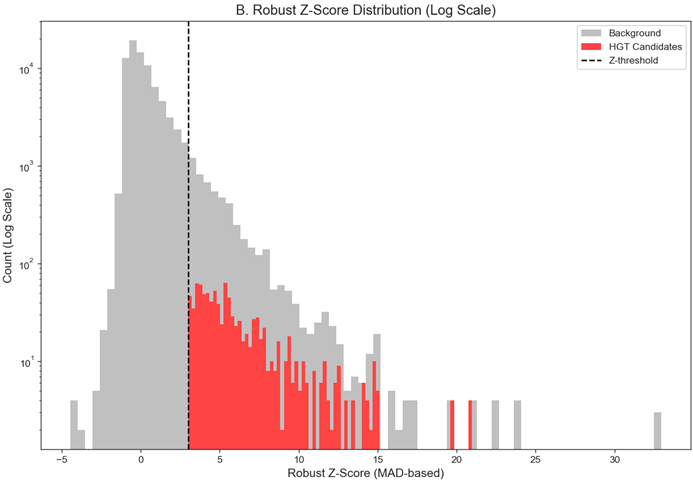
\includegraphics[width=0.55\linewidth]{figures/z_score_distribution.png}
    \caption{Distribution of MAD-based $z$-scores for all protein--protein edges, plotted on a logarithmic $y$-axis. The background distribution (grey) represents the global set of 911,306 edges, which clusters near the median ($z \approx 0$), reflecting expected evolutionary divergence consistent with vertical inheritance. The dashed black line marks the statistical significance threshold ($z = 3$). Edges connected to the final HGT candidates (red) are localized to the right tail of the distribution, confirming that GraFT concentrates its attention on a small fraction of edges that deviate strongly from species-pair baselines.}
    \label{fig:zscoredist}
\end{figure}

The full candidate graph contains 911,306 cross-species edges over 214,136 proteins. After Jaccard-based pre-pruning it contains 92,790 edges over 37,421 proteins across 5,262 connected components.

Component size is highly skewed: median size is 4 proteins, 95th percentile is 20, and the largest component contains 107 proteins. Median components span two species, and only 18.5\% contain $\ge 5$ species. This skewed distribution is consistent with the expectation that most proteins have narrow cross-species similarity (reflecting either no transfer or transfer limited to a few closely related pairs), while a small fraction participate in broad multi-taxon patterns.

Anomalous similarity is globally sparse: the median fraction of high-$z$ edges per component is 0, and only 3.9\% of components show substantial anomaly concentration (high-$z$ frac $> 0.3$). This sparsity is also evident in the global edge distribution (Figure~\ref{fig:zscoredist}), where most similarities cluster near the species-pair baseline while high-$z$ edges occupy a small right tail.

Across 37,421 proteins in the pruned graph, only 5.9\% satisfy the gating criteria (Section~\ref{subsubsec:gates}) and receive a non-zero score, indicating strong selectivity. Broad connectivity alone is insufficient: strong candidates require both taxonomic diversity within their component and concentrated anomalous similarity in their incident edges.

\subsection{Structural Regimes in the Jaccard-Pruned Graph}

Although most connected components are small and contain no anomalous edges, a small number of large multi-species components concentrate a substantial fraction of the signal. Table~\ref{tab:components} presents extended statistics for the three most prominent components.

\begin{table}[ht]
\centering
\small
\setlength{\tabcolsep}{4pt}
\resizebox{\linewidth}{!}{%
\begin{tabular}{lrrrrrrrrrrr}
\toprule
ID & Proteins & Edges & Density & Species & $H_{\mathrm{norm}}$ & high-$z$ frac & high-$z$ edges & max $z$ & top-10 $\bar{z}$ & sp.~pairs & top pair \% \\
\midrule
\hypertarget{tabrow:comp5}{5}  & 97 & 632 & 0.136 & 50 & 0.998 & 0.604 & 382 & 19.81 & 16.90 & 177 & 0.6 \\
\hypertarget{tabrow:comp8}{8}  & 95 & 589 & 0.132 & 49 & 0.998 & 0.467 & 275 & 15.71 & 14.26 & 168 & 0.7 \\
\hypertarget{tabrow:comp32}{32} & 71 & 332 & 0.134 & 31 & 0.958 & 0.063 &  21 &  5.75 &  4.61 &  99 & 4.2 \\
\bottomrule
\end{tabular}%
}
\caption{Extended summary statistics for the three most prominent connected components in the Jaccard-pruned similarity graph. Component IDs correspond to internal graph component identifiers. \textit{Column definitions:} Proteins $=|V_C|$; Edges $=|E_C|$; Density $=2|E_C|/(|V_C|(|V_C|-1))$; Species $=|\mathcal{S}_C|$; $H_{\mathrm{norm}}=H/\ln|\mathcal{S}_C|$ with $H=-\sum_{s\in\mathcal{S}_C}p_s\ln p_s$; high-$z$ frac $=|\{e:z_e\ge 3\}|/|E_C|$; high-$z$ edges $=|\{e:z_e\ge 3\}|$; top-10 $\bar{z}$ $=$ mean $z$ of the 10 highest-$z$ edges; sp.~pairs $=$ number of represented species pairs; top pair \% $=$ percentage of edges belonging to the most frequent species pair.}
\label{tab:components}
\end{table}

These three components illustrate qualitatively distinct structural regimes. Component 5 is a dense, high-entropy module with the strongest anomaly concentration. Component 8 has a chained topology in which compact subclusters are linked by few very high-surprise edges. Component 32 shows lower overall anomaly concentration, with signal mainly confined to specific bridging edges. Together, these regimes suggest that the graph captures different types of transfer-like patterns simultaneously.

\subsection{Component 5: Broad Multi-Taxa Exchange Module (Ribosomal Proteins S21 \& S12)}
\label{subsec:comp5}

\begin{figure}[!t]
  \centering
  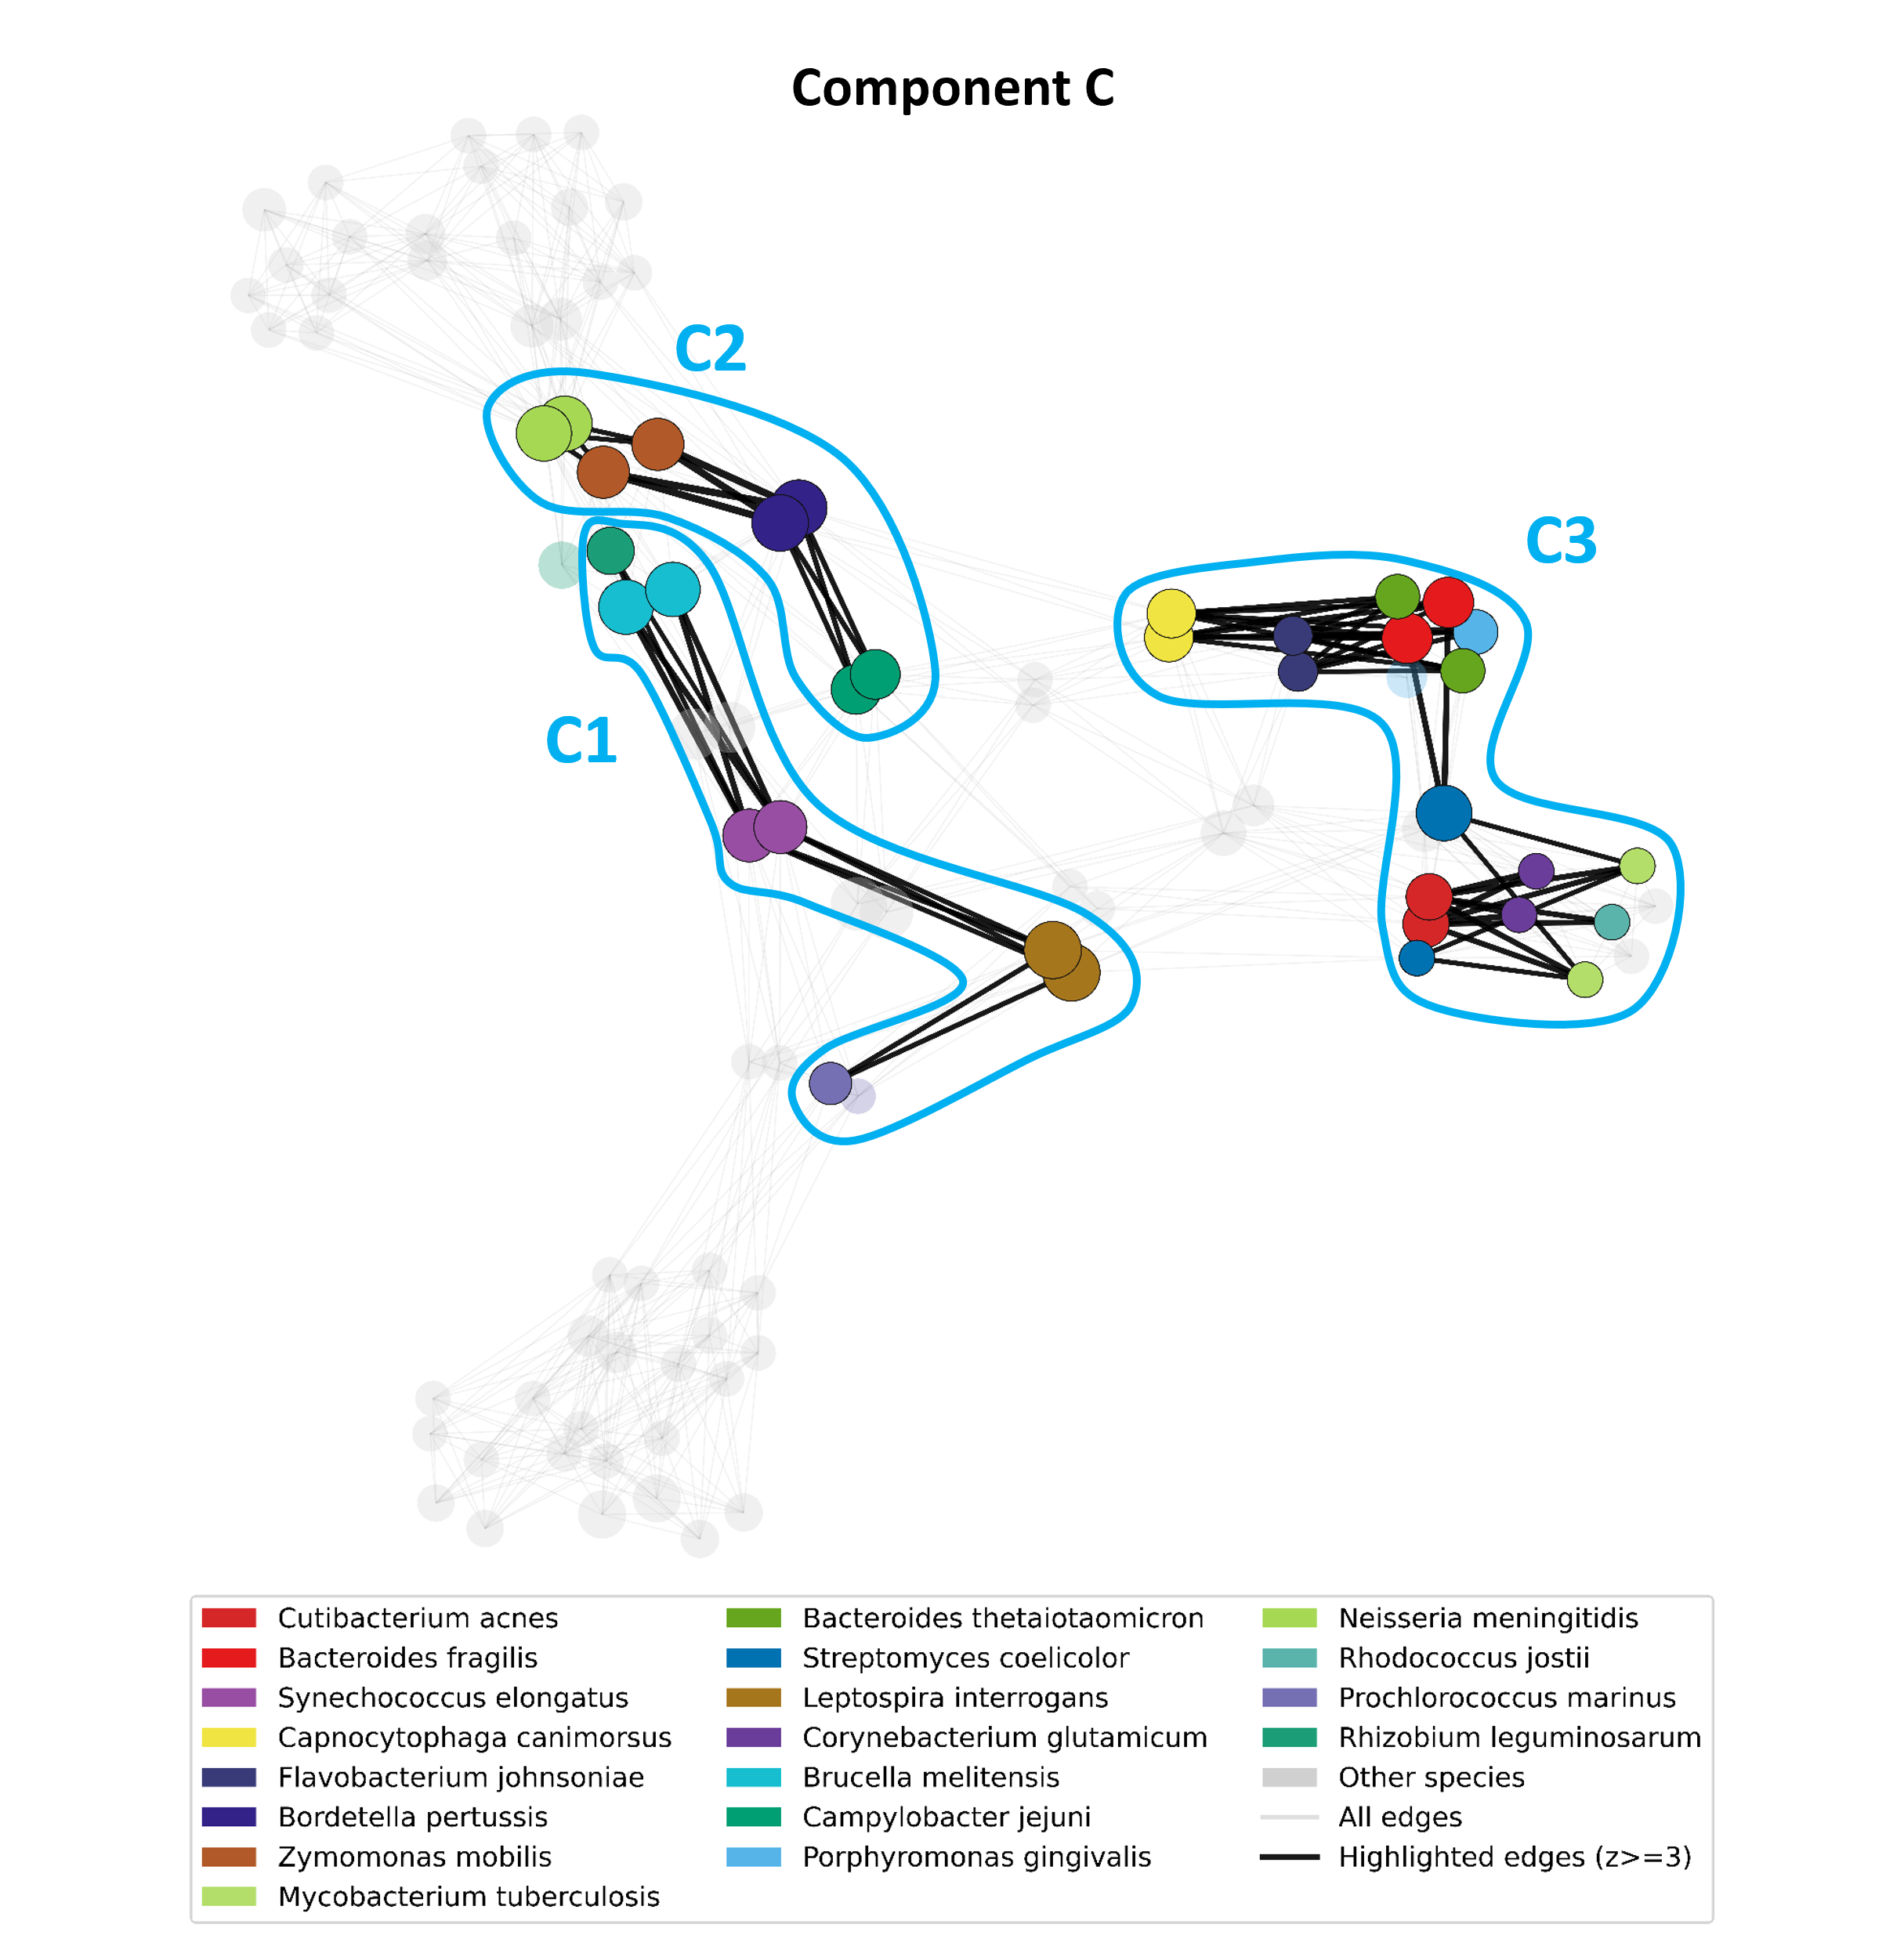
\includegraphics[height=0.45\textheight]{figures/component_C.png}
  \caption{Component 5: broad multi-taxa exchange module comprising 97 proteins across 50 species. Each node represents a protein colored by species. Bold edges denote statistically anomalous similarities ($z \ge 3$). The high-scoring proteins appear throughout the network and interact across many species simultaneously, consistent with a multi-species gene pool shaped by repeated HGT events\cite{compCShape}.}
  \label{fig:component5}
\end{figure}

Component 5 (97 proteins, 50 species, $H_{\mathrm{norm}}=0.998$, high-$z$ frac $= 0.604$, max $z=19.81$) is the component with the strongest and most widespread anomaly signal. The near-maximal species entropy ($H_{\mathrm{norm}} \approx 1$) indicates that proteins from all 50 species are represented roughly equally; the extremely high anomaly fraction (60.4\% of edges are high-$z$) indicates that the overwhelming majority of cross-species connections in this component deviate strongly from species-pair baselines. The top pair percentage of 0.6\% confirms that no single species pair dominates the edges, consistent with a broad multi-taxon exchange module rather than a bilateral transfer event.

The component comprises two distinct biological signals. Cluster $C_1$ consists entirely of ribosomal protein S21, which has been linked to late-stage phage replication: once acquired via HGT, S21 becomes part of the phage's genetic toolkit for hijacking host translational machinery to favor phage protein synthesis during late infection\cite{phage_S21_hgt}. This finding is consistent with results from independent HGT detection tools\cite{other_hgt_tool}.

Clusters $C_2$ and $C_3$ correspond to ribosomal protein S12 (encoded by \textit{rpsL}) within the 30S ribosomal subunit. Mutations in \textit{rpsL} are among the best-characterized mechanisms of streptomycin resistance\cite{Xu2025}: the protein forms part of the drug binding site and specific substitutions reduce binding affinity. Horizontal transfer of the \textit{rpsL} gene would directly confer streptomycin resistance to recipient organisms, providing a strong selective advantage under antibiotic pressure.

\subsection{Component 8: Chained Cross-Species Connectivity (30S Ribosomal Protein S10)}
\label{subsec:comp8}

\begin{figure}[!t]
  \centering
  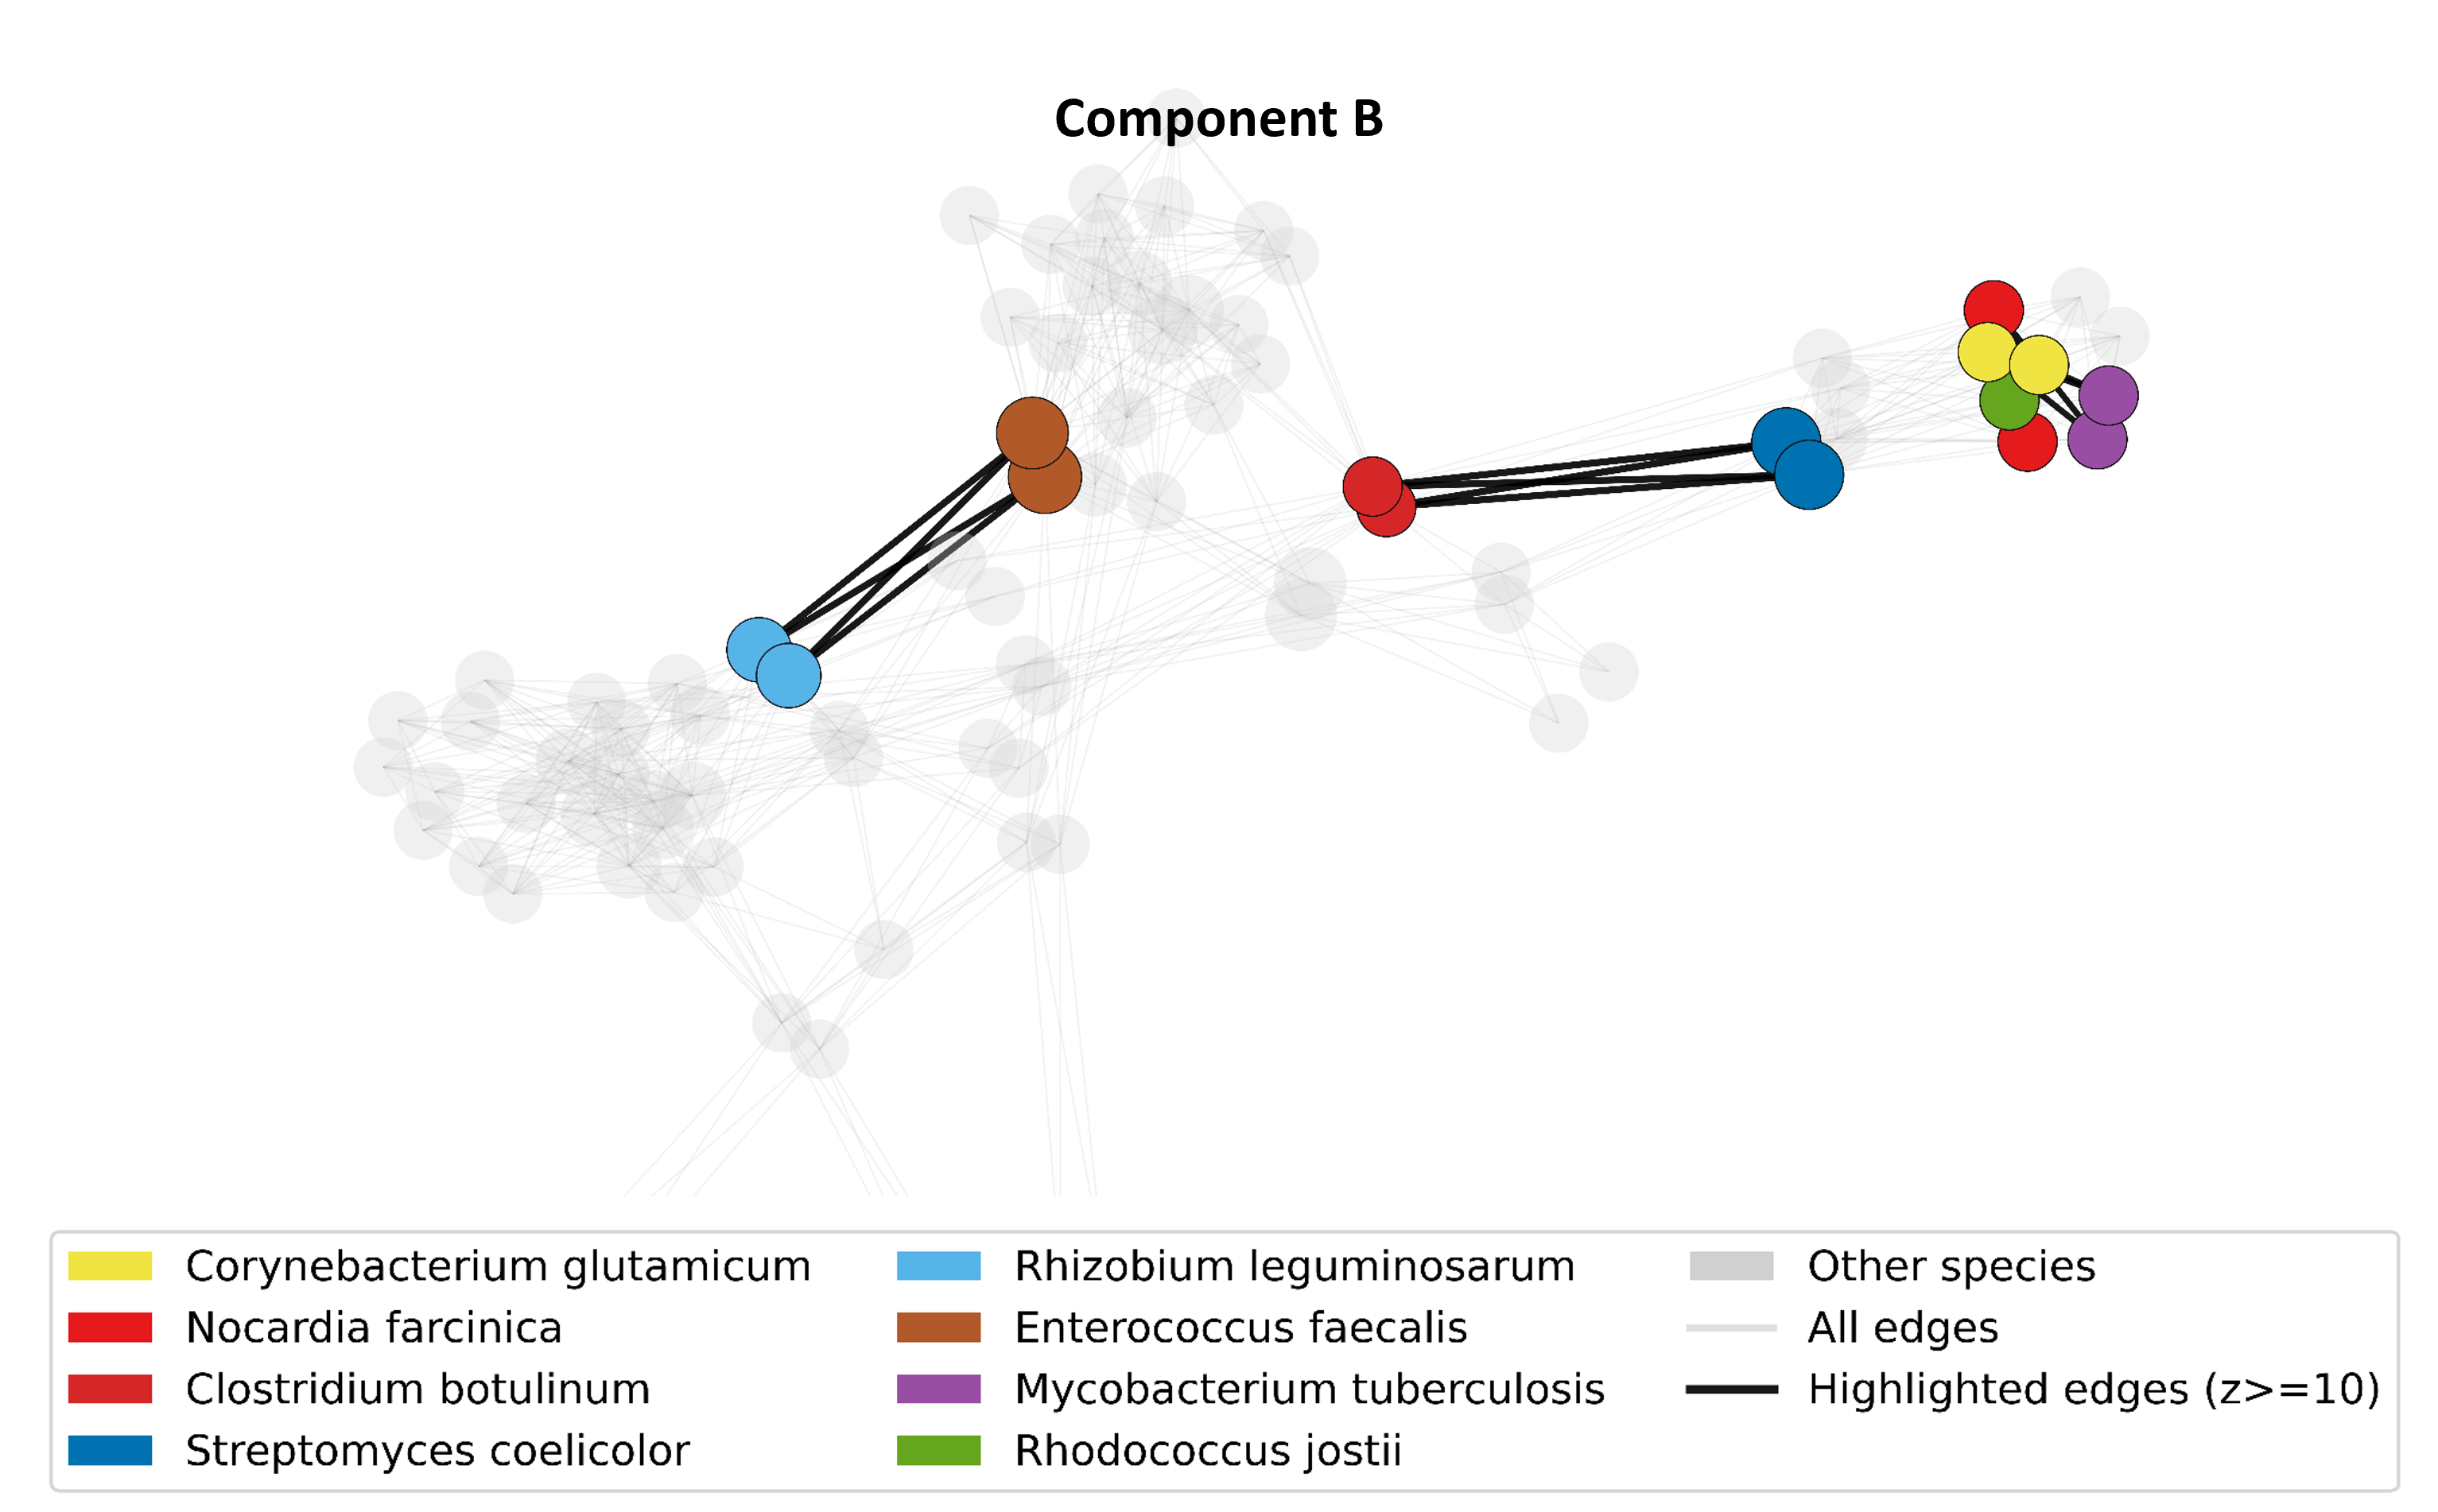
\includegraphics[height=0.45\textheight]{figures/component_B.png}
  \caption{Component 8: chained topology with 95 proteins across 49 species. Compact within-species subclusters are linked by a small number of extremely high-surprise inter-cluster edges. Bold edges denote statistically anomalous similarities (threshold raised to $z \ge 10$ for visualization, because $z$-scores in this component are exceptionally large; max $z=15.71$).}
  \label{fig:component8}
\end{figure}

Component 8 (95 proteins, 49 species, $H_{\mathrm{norm}}=0.998$, high-$z$ frac $= 0.467$, max $z=15.71$) shows a structurally distinct topology from Component 5. Rather than a single densely mixed module, the component is organized into compact within-species subclusters connected by a small number of bridging edges with extremely large $z$-scores. The top-10 mean $z$ of 14.26 and max $z$ of 15.71 are the largest in the dataset, indicating that the inter-cluster edges deviate from species-pair baselines by an extraordinary margin---approximately 15 robust standard deviations above the species-pair median. The top pair percentage of 0.7\% again rules out a single dominant bilateral transfer.

All clusters in Component 8 correspond to the 30S ribosomal protein S10, encoded by \textit{rpsJ}. Mutations in \textit{rpsJ} are known markers of tigecycline resistance, a broad-spectrum tetracycline antibiotic used as a last-resort treatment\cite{antibiotic_res,antibiotics12091367}, making this gene a high-value target under antibiotic pressure. Horizontal transfer of \textit{rpsJ} has been reported among \textit{Mycobacterium} species, including \textit{M.~tuberculosis}\cite{mycobacterium_rpsJ_transfer}, a pathogen of major global health importance. The chained topology of Component 8---where subclusters from different species are bridged across large taxonomic distances---is consistent with a relay-like transfer pattern in which the gene has moved sequentially through intermediate hosts.

\subsection{Component 32: Localized High-Confidence Bridges (Glucose-1-Phosphate Thymidylyltransferase)}
\label{subsec:comp32}

\begin{figure}[!t]
  \centering
  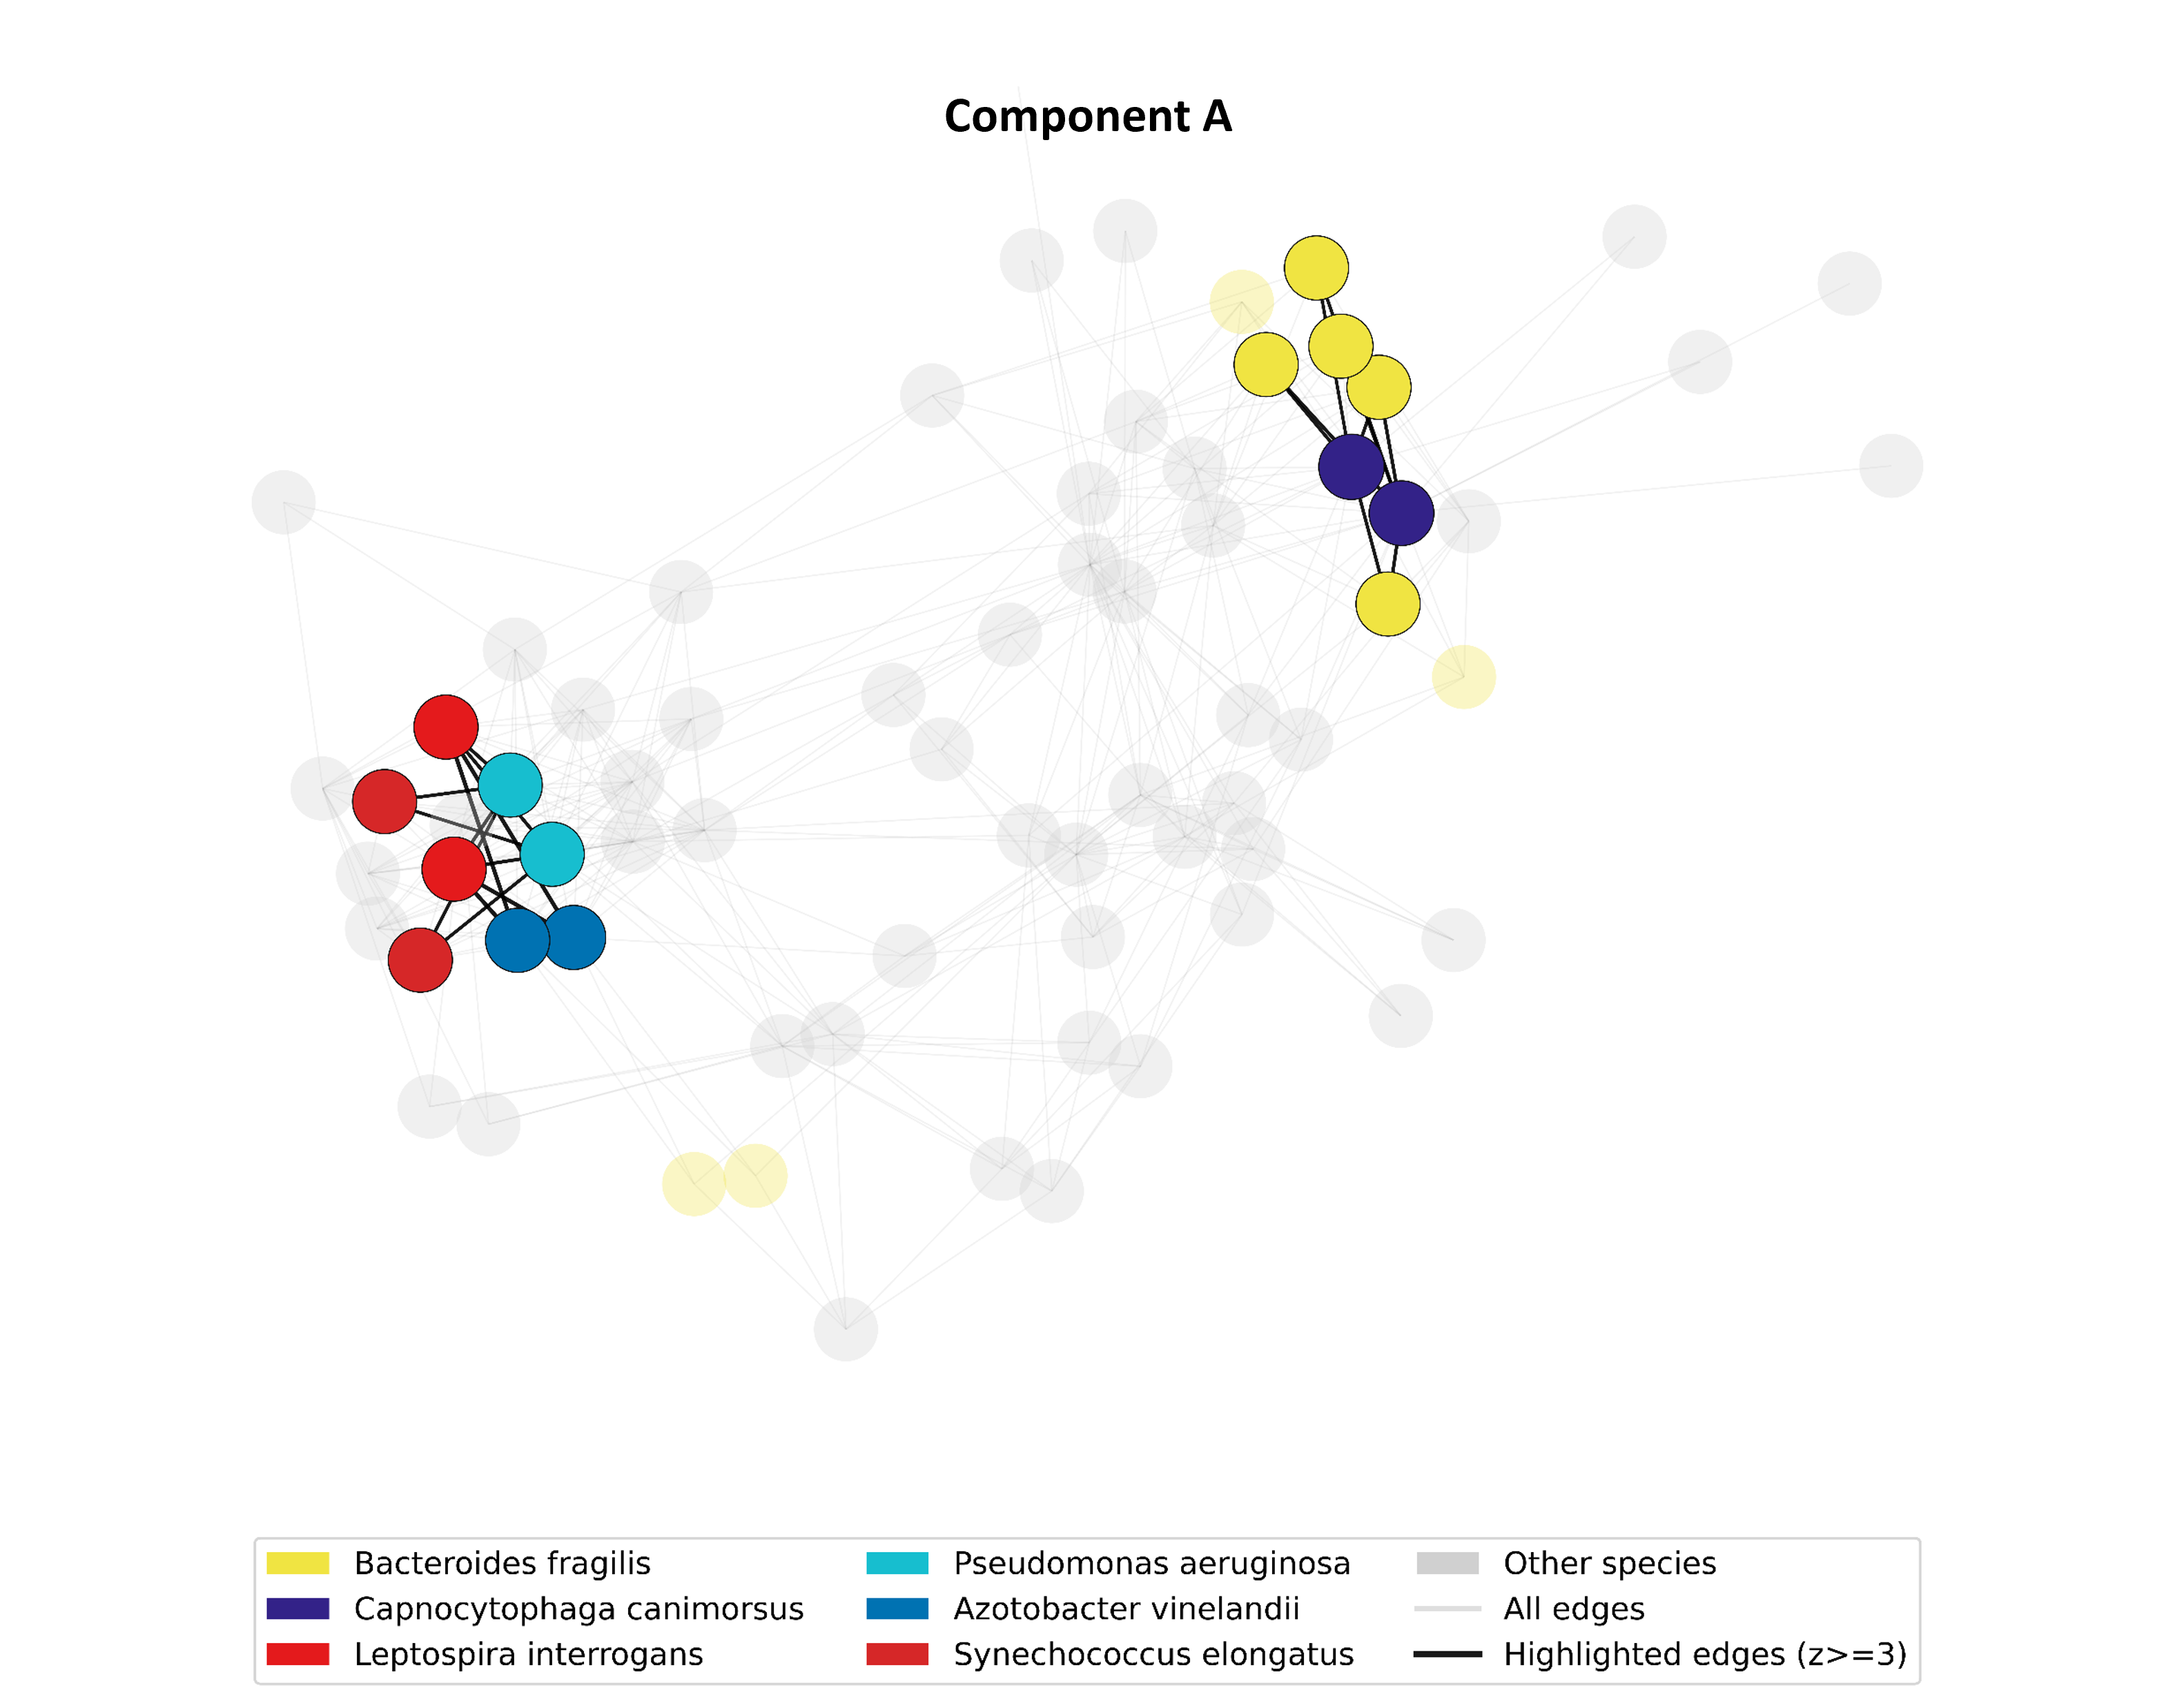
\includegraphics[width=\linewidth]{figures/component_A.png}
  \caption{Component 32: localized high-confidence bridges. 71 proteins across 31 species ($H_{\mathrm{norm}}=0.958$). Two coherent regions are connected by a small number of strong cross-species edges, with anomalous signal concentrated in the bridging edges (high-$z$ frac $= 0.063$, max $z=5.75$). Bold edges denote statistically anomalous similarities ($z \ge 3$).}
  \label{fig:component32}
\end{figure}

Component 32 (71 proteins, 31 species, $H_{\mathrm{norm}}=0.958$, high-$z$ frac $= 0.063$, max $z=5.75$) is qualitatively different from Components 5 and 8. The overall anomaly fraction is low (only 6.3\% of edges are high-$z$), but the signal is highly localized to specific bridging edges that connect otherwise coherent species clusters. The top pair percentage of 4.2\% (compared to 0.6--0.7\% for Components 5 and 8) indicates that a single species pair accounts for a substantial share of the anomalous edges, suggesting a more focused bilateral or limited-range transfer event rather than a broad multi-taxon exchange.

Both clusters in Component 32 correspond to glucose-1-phosphate thymidylyltransferase, a key enzyme in the biosynthesis of bacterial surface polysaccharides. These polysaccharide structures contribute to host immune evasion: for example, \textit{Capnocytophaga} species (pathogenic oral commensals in dogs that can infect immunocompromised humans) use surface polysaccharides to resist the bactericidal effects of human serum, providing a major virulence advantage\cite{CompA1,CompA2,CompA3}. Horizontal transfer of polysaccharide biosynthesis enzymes thus represents an important mechanism for acquiring immune evasion capabilities.

\subsection{Comparison with the Full Candidate Graph}

To quantify the effect of pre-pruning, we compared the Jaccard-pruned graph against the full candidate graph produced before the species-pair quantile and degree filters (Table~\ref{tab:full_vs_pruned}). The full graph contains 9.8-fold more edges and 5.7-fold more proteins, with a higher mean degree. More importantly for interpretation, the full graph contains a giant connected component of 41,509 proteins and 224,120 edges spanning all 50 species, whereas the largest component after pruning contains 107 proteins and 374 edges.

\begin{table}[ht]
\centering
\small
\setlength{\tabcolsep}{5pt}
\resizebox{\linewidth}{!}{%
\begin{tabular}{lrrrrrrr}
\toprule
Graph & Edges & Proteins & Mean degree & Components & Largest comp. proteins & Largest comp. edges & Largest comp. high-$z$ frac \\
\midrule
Full candidate & 911,306 & 214,136 & 8.51 & 17,238 & 41,509 & 224,120 & 0.043 \\
Jaccard-pruned & 92,790 & 37,421 & 4.96 & 5,262 & 107 & 374 & 0.005 \\
\bottomrule
\end{tabular}%
}
\caption{Structural comparison of the full candidate graph and the Jaccard-pruned graph. Mean degree is $2|E|/|V|$. The high-$z$ fraction is computed within the largest connected component of each graph using the same species-pair robust normalization threshold ($z \ge 3$).}
\label{tab:full_vs_pruned}
\end{table}

The full graph's giant component still contains statistically anomalous edges (9,702 high-$z$ edges), but they are diffuse, accounting for only 4.3\% of edges in that component. By contrast, the pruned components analyzed above isolate much more concentrated anomaly regimes, including Component~5 (60.4\% high-$z$ edges) and Component~8 (46.7\%). Thus, pre-pruning is not merely a computational downsampling step: it separates the broad background of conserved cross-species similarity into smaller modules in which anomalous edges and component boundaries are more interpretable. The Jaccard-based quantile filter therefore acts as a quality-control step that preserves the top tier of cross-species similarity within each species pair while discarding the background mass of moderate-similarity edges.

\subsection{Score Distribution and Selectivity}

Among the top 200 ranked proteins, the median score was 5.9 (IQR: 4.47--8.17), with the 95th percentile at 12.74 and a maximum of 18.76. These values represent the extreme upper tail of the scoring distribution among the 5.9\% of proteins that passed gating. The right-skewed distribution of scores reflects the log-space construction of $S(u)$, where multiple co-occurring anomaly signals combine multiplicatively: proteins that score extremely high are those where all six multiplicative factors simultaneously take large values, a condition that is rare but interpretable.

\FloatBarrier

% =========================
% 5. Limitations and Detectability of Ameliorated HGT
% =========================
\section{Limitations and Detectability of Ameliorated HGT}
\label{sec:amelioration}

\begin{figure}[ht]
    \centering
    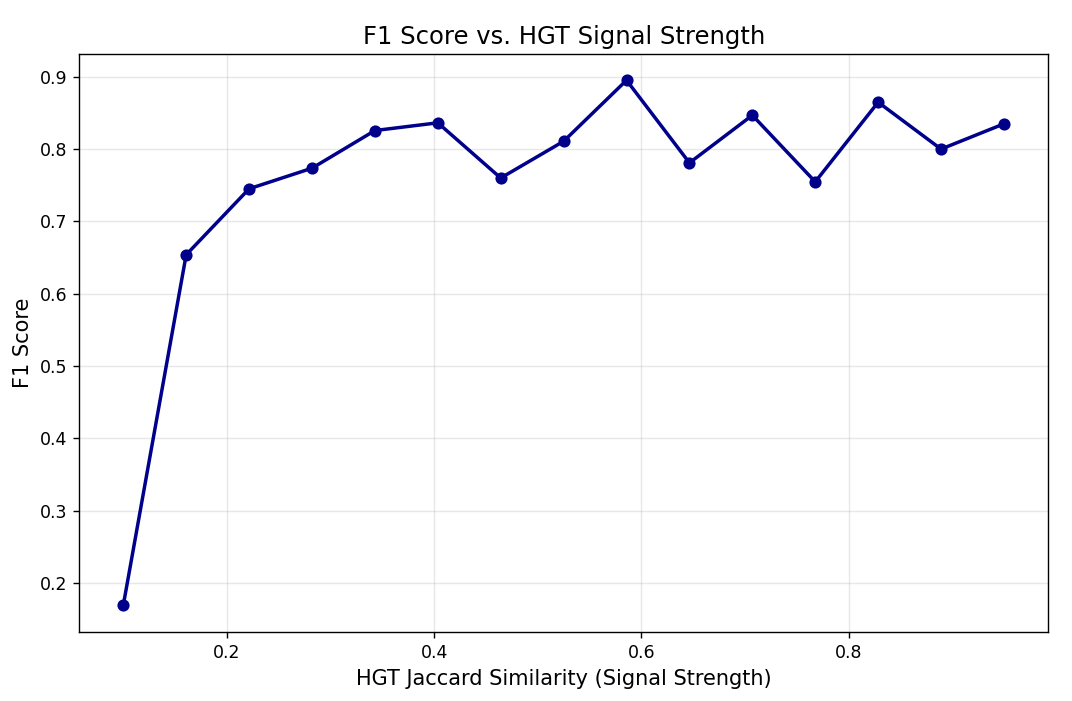
\includegraphics[width=0.65\linewidth]{figures/f1.png}
    \caption{$F_1$ score of GraFT as a function of injected HGT Jaccard similarity, used as a proxy for the degree of genomic amelioration. Each point represents an independent simulation with 10 species (50 proteins per taxon) and 30 injected HGT events, alongside conserved housekeeping genes (Jaccard 0.75--0.95) and background proteins (low Jaccard). The method achieves stable performance ($F_1 \ge 0.75$) for Jaccard similarity $\ge 0.20$ but degrades rapidly below this threshold, indicating substantially reduced sensitivity for highly ameliorated transfers.}
    \label{fig:amelioration_f1}
\end{figure}

To assess how genomic amelioration affects detectability, we simulated HGT events with varying Jaccard similarity while controlling for conserved housekeeping genes (high Jaccard) and background proteins (low Jaccard). Because GraFT's candidate generation and pruning stages prioritize high-similarity edges, strongly ameliorated transfers---those where the transferred gene has accumulated many substitutions after transfer---are increasingly classified as background and discarded.

As shown in Figure~\ref{fig:amelioration_f1}, performance is stable ($F_1 \ge 0.75$) for Jaccard similarities $\ge 0.20$ but degrades rapidly below this threshold. This is an inherent limitation of any \textit{k}-mer overlap approach: post-transfer sequence divergence reduces the number of shared hexapeptide \textit{k}-mers below the thresholds required for candidate generation and pruning. The method therefore primarily detects relatively recent or slowly-evolving HGT events where the sequence similarity with the donor lineage remains detectable.

Classical alignment-based and phylogenetic methods may retain sensitivity at lower similarity, but at much greater computational cost and with sensitivity to alignment quality. The alignment-free approach occupies a complementary niche: high-throughput screening of high-similarity (recent or slowly-evolving) transfers, with the expectation that older, more diverged events require orthogonal validation methods.

% =========================
% 6. Discussion
% =========================
\section{Discussion}
\label{sec:discussion}

\subsection{Summary}

GraFT is intended as a scalable hypothesis-generation framework rather than a definitive test for horizontal gene transfer. By replacing alignment and phylogenetic reconstruction with species-aware normalization and graph-structural analysis, we trade resolution for scalability, prioritizing candidates for downstream validation rather than directly confirming transfer events.

Across the three prominent components identified---spanning 50, 49, and 31 species respectively---all candidates are supported by independent biological literature, and all are associated with known fitness advantages (antibiotic resistance in the case of S12/rpsL, S10/rpsJ, or immune evasion in the case of glucose-1-phosphate thymidylyltransferase) that would provide strong selective pressure for HGT fixation.

The consistency of signal across edge-level anomaly ($z$-scores), node-level connectivity (degree, betweenness), and component-level taxonomic mixing (species entropy) suggests that high-ranking candidates are not artifacts of any single heuristic. Instead, they represent multi-scale structural deviations from expected background similarity, which is precisely the signature we would expect from genuine horizontal transfer events.

\subsection{Design Choices and Trade-Offs}

Several design choices reflect explicit trade-offs between sensitivity and specificity. Restricting candidate generation ($k=6$, $\ge 6$ shared \textit{k}-mers, posting lists $\le 100$, top-10 matches per protein) suppresses conserved motifs and ubiquitous housekeeping genes. While this substantially reduces false positives arising from generic conservation, it may also exclude true transfer events involving highly conserved or short protein domains. Similarly, per-species-pair percentile pruning (top 10\%) and degree capping (top 20 edges per node) improve structural interpretability but introduce heuristic thresholds that may affect sensitivity in underrepresented species pairs.

The robust $z$-score normalization mitigates heterogeneity across species pairs, yet its effectiveness depends on sufficient edge counts per pair (minimum 30). Rare species pairs with few observations may therefore yield unstable baselines. In addition, the anomaly threshold ($z \ge 3$) emphasizes extreme deviations and may bias the ranking toward dramatic cross-species similarities while overlooking subtler but biologically meaningful transfers.

The taxonomic distance filter (range $[2,4]$) is a deliberate approximation: it excludes intra-genus comparisons (distance $< 2$) where high similarity is expected and does not indicate cross-species transfer, and very distant comparisons (distance $> 4$) where \textit{k}-mer overlap is typically too sparse to yield reliable signal. This filter may inadvertently exclude real transfers between very closely related genera or across phylum boundaries.

\subsection{Sources of False Positives and False Negatives}

False positives may arise from convergent evolution producing functional analogs with similar sequences, ancient homologs maintained by strong purifying selection across deep evolutionary time, unmodeled taxonomic structure (e.g., two sampling units treated as distinct ``species'' that are genomically nearly identical), or contamination and assembly artifacts in the RefSeq genomes.

Conversely, false negatives may arise when transfer events occur between closely related taxa filtered by the taxonomic distance threshold, when post-transfer divergence reduces \textit{k}-mer overlap below detection limits (the amelioration problem discussed in Section~\ref{sec:amelioration}), or when the transferred protein is too short or lacks sufficient unique \textit{k}-mers to form high-Jaccard edges with source proteins.

\subsection{Multi-Assembly Redundancy}
\label{subsec:redundancy}

Selecting up to two assemblies per species introduces redundancy: near-identical assemblies of the same species will produce many high-similarity cross-assembly edges that may inflate statistics for some species pairs. This could affect the robustness of MAD-based normalization for species pairs with many near-identical proteins. Future versions of the pipeline should consider stricter de-duplication or single-assembly-per-species selection to mitigate this effect.

\subsection{Future Directions}

\paragraph{Validation.} The most valuable next step is validation against curated HGT benchmarks (e.g., HOGENOM, HGTree) or established HGT detection tools to enable quantitative precision/recall evaluation at scale. The simulations in Section~\ref{sec:amelioration} are a first step but use a simplified generative model; real HGT events involve complex evolutionary dynamics that are not captured by a single Jaccard similarity parameter.

\paragraph{Scaling.} Sketching approaches such as MinHash\cite{Broder1997,Ondov2016} could replace exact Jaccard computation in the candidate generation step, reducing the computational cost of large-scale similarity screening while maintaining approximate Jaccard estimates. This would enable application to datasets orders of magnitude larger than the current 324,000-protein testbed.

\paragraph{Sensitivity analysis.} Sensitivity analysis over the hyperparameters ($k$, pruning percentiles, anomaly thresholds, gating criteria) would clarify robustness and identify which parameters most strongly influence candidate ranking. Given the many heuristic choices in the pipeline, understanding their individual impact is important for both method validation and principled adaptation to new datasets.

\paragraph{Orthogonal validation signals.} Future validation should integrate orthogonal genomic evidence, including synteny conservation, plasmid or genomic island association, phylogenetic incongruence analysis (gene tree vs. species tree), and GC-content or codon usage anomaly detection. Combining these signals with graph-structural candidates would increase confidence in prioritized events and reduce the false positive rate.

\paragraph{Unified hierarchical pipeline.} An attractive extension is a hierarchical pipeline in which GraFT serves as a broad first-pass screening layer, and alignment-based phylogenetic analysis is applied only to the small set of high-priority candidates identified by graph scoring. This would combine the scalability of \textit{k}-mer methods with the resolution of phylogenetic reconstruction, while limiting the computational cost of alignment to the subset of proteins where it is most needed.

\paragraph{Broader scope.} Finally, the framework could be extended to eukaryotic datasets (e.g., horizontal gene transfer between bacteria and unicellular eukaryotes\cite{Soucy2015}), cross-kingdom comparisons, or viral genomes where HGT-like events (recombination, reassortment) are prevalent.

\subsection{Implementation and Reproducibility}

All scripts required to reproduce GraFT are available in the GitHub repository linked on the title page. The repository contains the exact configurations, intermediate artifacts, and visualization code used to produce our results, along with online supplementary material including extended result tables and additional component visualizations. The full scoring derivation presented in Section~\ref{sec:scoring} corresponds exactly to the implemented code, ensuring that the mathematical specification is a faithful description of the pipeline rather than an idealized summary.

% =========================
% 7. Conclusion
% =========================
\section{Conclusion}

We presented GraFT, a scalable, alignment-free framework for large-scale HGT candidate detection based on species-pair--aware normalization and sparse protein similarity graphs. By combining robust statistical calibration with graph-structural features and explicit multi-criteria gating, the method selectively reduces a collection of approximately 324,000 proteins to a compact, interpretable set of high-priority candidates suitable for downstream phylogenetic and genomic validation.

The three prominent components identified---spanning 50, 49, and 31 species---each correspond to biologically plausible HGT candidates with established fitness advantages: streptomycin resistance (ribosomal protein S12/rpsL), tigecycline resistance (ribosomal protein S10/rpsJ), and serum resistance via surface polysaccharides (glucose-1-phosphate thymidylyltransferase). The full formal scoring framework, presented in Section~\ref{sec:scoring}, enables transparent, reproducible, and tunable candidate prioritization. Graph-based structural context, when combined with species-pair--aware normalization, provides a powerful signal for separating genuine cross-species transfer patterns from the background of conserved protein similarity.

% =========================
% Author Contributions

%\section*{Author Contributions}
%\addcontentsline{toc}{section}{Author Contributions}

%Roee Tekoah led the method design, implementation, experimental analysis, scoring formalization, visualization and reproducibility infrastructure, and manuscript writing. Noam Korkos contributed pruning-code and biological validation and interpretation of candidate components. Both authors reviewed the manuscript.
% =========================

% =========================
% References
% =========================
\bibliographystyle{unsrt}
\bibliography{references}

\end{document}
